\chapter{大动量希格斯粒子的产生和到WW散射的物理}
\label{chap2}
\fontsize{12bp}{14.4pt}

\section{希格斯粒子的产生和衰变}
\subsection{希格斯粒子的产生}


在标准模型中,夸克、轻子、W、Z玻色子都通过希格斯机制被赋予质量。

LHC以及下一代对撞机实验的重要目标之一就是研究测量希格斯粒子的相关性质

\begin{table}[htbp]
    \caption{标准模型中希格斯粒子的产生道和相关参数}\label{table:2.1}
    \centering
    \begin{tabular}{>{\centering\arraybackslash}p{2cm}%
    >{\centering\arraybackslash}p{7cm}%
    >{\centering\arraybackslash}p{2cm}%
    >{\centering\arraybackslash}p{2cm}}
    \toprule\toprule
    \textbf{产生道} & \textbf{产生方式} & \textbf{分支比} & \textbf{截面}\\
    \midrule
    ggF & 胶子通过b/top夸克圈聚合产生 & $\sim 87\%$ & \SI{48.5}{pb}\\
    VBF & W/Z矢量玻色子聚合产生 & $\sim7\%$ & \SI{3.78}{pb}\\
    WH & W/Z矢量玻色子与希格斯联合产生 & $\sim 4\%$ & \SI{1.37}{pb}\\
    ttH & 正反top夸克与希格斯联合产生 & $\sim1\%$ & \SI{0.51}{pb}\\
    bbH & 正反bottom夸克与希格斯联合产生 &  $\sim 1\%$ & \SI{0.49}{pb}\\
    tH & t,b,$q^\prime$与希格斯联合产生 & $\sim 0.1\%$ & \SI{0.09}{pb}\\
    \bottomrule\bottomrule
\end{tabular}
\end{table}
每个产生道都有独特的拓扑结构,对于其中的稀有道,尽管很难探测,却是研究超出标准模型的重要场景。

\subsection{希格斯粒子的衰变}
\begin{table}[htbp]
    \caption{标准模型中希格斯粒子的衰变道和相关参数}\label{table:2.1}
    \centering
    \begin{tabular}{>{\centering\arraybackslash}p{2cm}%
    >{\centering\arraybackslash}p{7cm}%
    >{\centering\arraybackslash}p{2cm}%
    >{\centering\arraybackslash}p{2cm}}
    \toprule\toprule
    \textbf{衰变道} & \textbf{主要衰变方式(领头阶)} & \textbf{分支比} & \textbf{稀有衰变}\\
    \midrule
    $H\to bb$ & 直接衰变 & $\sim 58.1\%$ & 否\\
    $H\to WW$ & 直接衰变,一个在壳一个离壳 & $\sim 21.5\%$ & 否\\
    $H\to\tau\tau$ & 直接衰变 & $\sim 6.26\%$ & 否\\
    $H\to ZZ$ & 直接衰变 & $\sim2.64\%$ & 否\\
    $H\to \gamma\gamma$ & 通过W/t/b/$\tau$圈间接衰变 &  $\sim0.23\%$ & 否\\
    $H\to\mu\mu$ & 直接衰变 & $\sim 0.022\%$ & 是\\
    $H\to Z\gamma$ & 通过W/t/b/$\tau$圈间接衰变 & $\sim 0.154\%$ & 是\\
    $H\to cc$ & 直接衰变 & $\sim2.88\%$ & 是\\
    $H\to gg$ & 通过top/bottom圈间接衰变 & $\sim 8.18\%$ & 是\\
    \bottomrule\bottomrule
\end{tabular}
\end{table}
对于其中五个非稀有衰变道,有以下性质:
\begin{itemize}
    \item $\gamma\gamma$和$ZZ\to4\ell$道:高分辨度和高信噪比,常用来精确测量希格斯质量和微分散射截面。
    \item $WW$道:高分支比,但衰变末态的中微子导致低信噪比和低分辨度。
    \item $\tau\tau$和$bb$道:高分支比,低信噪比,用于直接探测希格斯粒子与费米子的耦合。
\end{itemize}

\section{大动量希格斯粒子}
\begin{enumerate}
    \item 可以提高标准模型希格斯测量的敏感度:在希格斯粒子$p_T>200$[GeV]的区域,$H\to bb$、$H\to\tau\tau$道可以从未分辨喷注的分析中获益;在更高的$p_T$区域,$H\to ZZ/WW\to 4q$也可以获益。
    \item 可以用作搜寻超出标准模型新物理的工具,包括:辐射子,Randall-Sundrum Bulk Graviton,复合希格斯粒子,新的矢量三重态,暗物质的探寻(2HDM)
\end{enumerate}

标准模型对希格斯粒子动量微分截面的高阶修正在高动量区十分稳定,次领头阶与领头阶的比值固定在一定值范围内;而部分超标准模型理论的这一比值则会随动量增大而发生较大的增长。所以对大动量区域希格斯粒子的研究可以用来探测出现高$p_T$区域的新物理。

\begin{figure}[H]
 \centering
 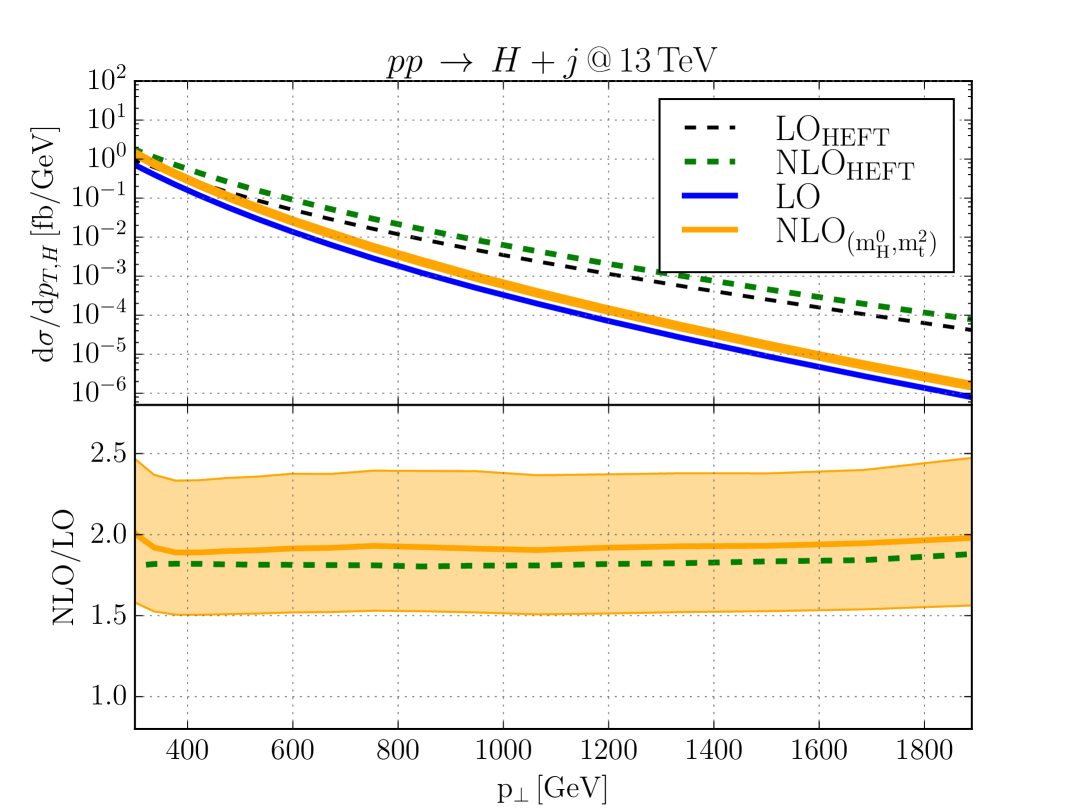
\includegraphics[height=8cm, width=11cm]{pictures/SM_NLO:LO.png}
  \caption{LHC上质心系能量为13TeV时希格斯玻色子的横向动量分布。上图显示标准模型和无穷大top质量有效场论(HEFT)中领头阶(LO)和次领头阶(NLO)的预测。下半部分显示了各自的NLO/LO校准比值。黄色边带表示由于尺度变化导致的标准模型结果的理论误差。}
 \label{fig:2.1}
\end{figure}

\begin{figure}[H]
 \centering
 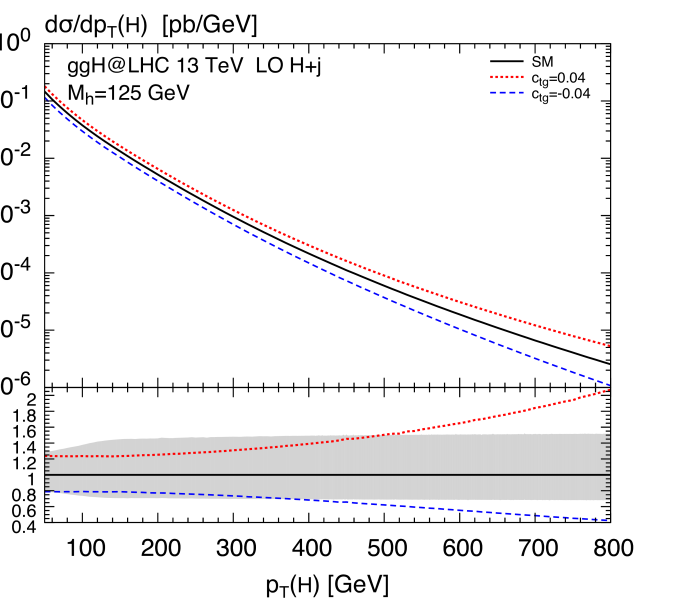
\includegraphics[height=10cm, width=11cm]{pictures/BSM_NLO:LO.png}
  \caption{超标准模型的chromomagnetic算符对在目前实验限制允许的区域内的希格斯玻色子谱分布。}
 \label{fig:2.2}
\end{figure}
区别:一个低$p_T$的玻色子衰变到两夸克,重建时看上去会像是两个喷注;但是对于重粒子衰变到两夸克时,两个夸克会被合并成一个喷注,这是因为重粒子的质量会变成两个W的大动量。

2012 年对希格斯玻色子的观察开辟了一种令人兴奋的方法,可以寻找标准模型之外的新物理学线索,这可能有助于阐明诸如暗物质的性质和物质-反物质不对称性等谜团。一种方法是直接寻找与希格斯玻色子对话的新粒子或寻找它的表亲,而另一种方法则依赖于测量它的属性并在标准模型中寻找与其预期属性的偏差,这是我们目前对粒子物理学的最佳描述。在 CMS 最近的这个结果中,物理学家探索了由高横向动量或大量洛伦兹助推产生的希格斯玻色子,以此作为刺激标准模型为我们提供潜在新物理学暗示的一种方式。

寻找能量增强的希格斯玻色子可以让物理学家间接地对质量尺度上的新物理学敏感,这些物理学可能太重而无法在大型强子对撞机上直接观察到。在量子场论中,这些间接暗示是虚拟产生的新粒子,这意味着它们只是瞬间出现和消失。这些虚拟的新粒子会导致作为横向动量函数产生的希格斯玻色子的数量或比率出现较大偏差。对于许多新的物理场景,与标准模型的最大偏差是最高的,但产生如此高能量的希格斯玻色子是非常罕见的。

\begin{figure}[H]
 \centering
 \caption{希格斯玻色子候选喷注的质量分布,红色填充是叠加在本底上的希格斯信号。}
 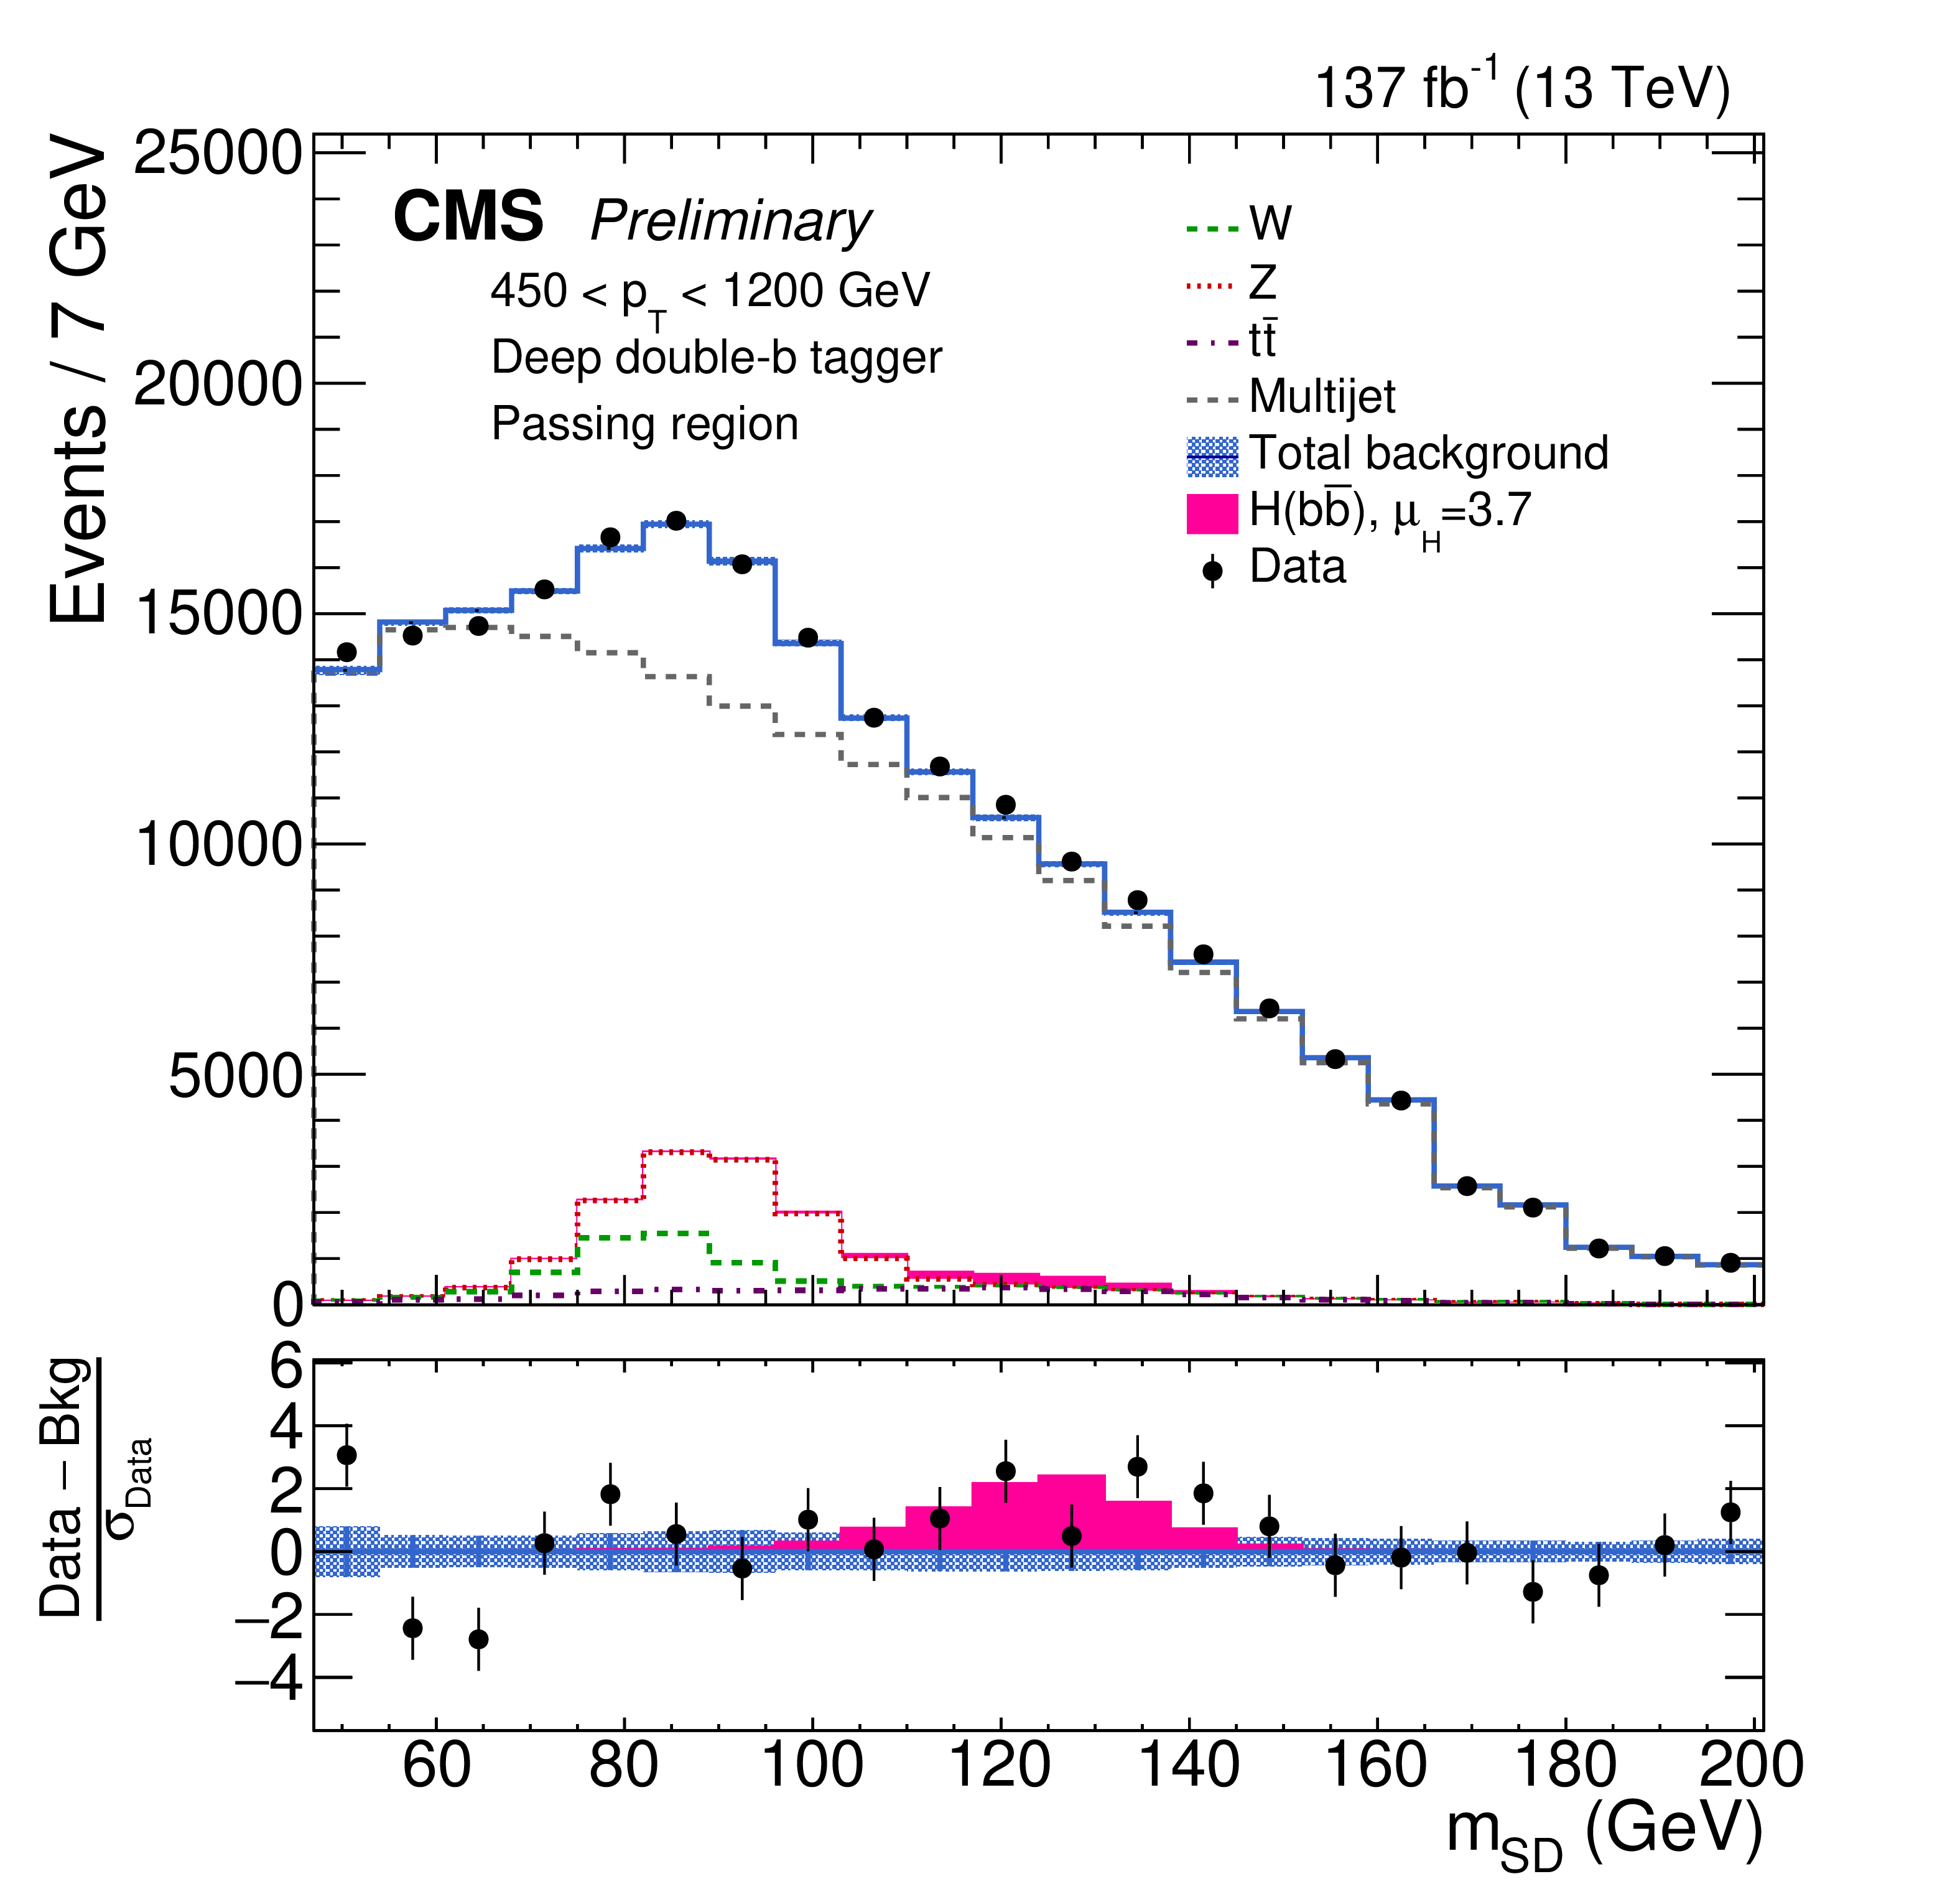
\includegraphics[height=10cm, width=10cm]{pictures/CMS-PAS-HIG-19-003_Figure_001-b.png}
 \label{fig:2.3}
\end{figure}

CMS 实验研究了横向动量高达 1200 GeV 的希格斯玻色子,这意味着希格斯玻色子以 99.5\% 或更高的光速传播,远远超出任何其他分析所探索的范围。这为与希格斯玻色子对话的新虚拟粒子提供了前所未有的灵敏度。下图显示了候选希格斯玻色子射流在所有分析选择后的质量分布。希格斯玻色子信号很小但可见(洋红色),其显着性为背景的 2.5 个标准偏差。在标准模型中,我们期望看到 0.7 个标准差。观察到的希格斯玻色子产生率高于预期,这使得结果很有趣,尽管在统计上并不显着,并且与新一批数据密切相关。 

展望未来,CMS 将通过研究具有其他希格斯衰变最终状态的高升压区域以及从 2021 年开始的第 3 轮运行更多数据,然后从 2027 年开始的高亮度 LHC 时代,继续获得更清晰的画面。增强的希格斯玻色子刚刚开始——敬请期待未来的结果,看看这部电影是如何结束的!  

\section{$H\to WW$的物理及动机}
LHC上最主要的$H\to WW$产生模式就是胶子聚合产生(ggF),如图所示。初态胶子通过top夸克圈耦合成希格斯粒子,然后希格斯粒子继续衰变成一对W玻色子。

次多产生模式是矢量玻色子聚合产生(VBF),如图所示,其生产截面大约比ggF小一个数量级。两个初态夸克辐射出W或Z玻色子,然后W或Z玻色子聚合成希格斯粒子,并进一步衰变成一对W玻色子。但VBF末态会生成两个喷注加一对W玻色子,而ggF只会生成一对W玻色子。

研究WW末态状态的主要动机是寻找希格斯玻⾊⼦。希格斯玻⾊⼦可以直接衰减为符号相反的W玻⾊⼦对。最重要的$\to WW$⽣产图,胶⼦聚变 (ggF) 图,如图所示。ggF生产过程是
\begin{figure}[H]
 \centering
 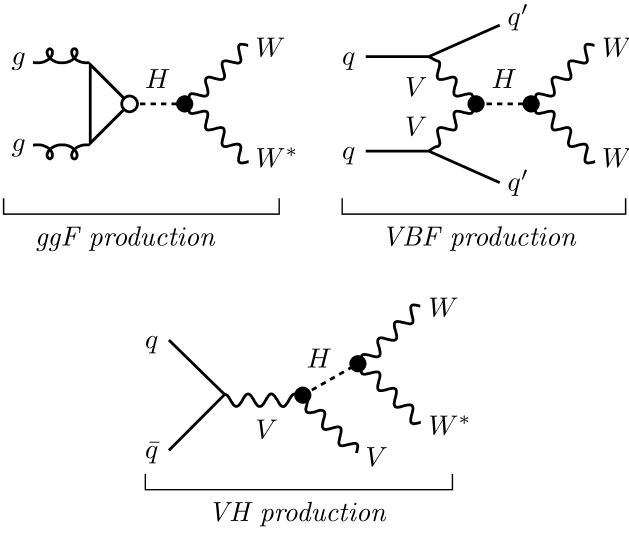
\includegraphics[height=10cm, width=12cm]{pictures/HWW_production.png}
  \caption{$H\to WW$的主要生产过程的领头阶费曼图:(a)通过夸克圈的ggF生产过程;(b)VBF生产过程,末态除了两个W玻色子之外还有两个夸克喷注;(c)VH联合产生,末态有三个玻色子}
 \label{fig:2.4}
\end{figure}

$H\to WW$产⽣的总速率由希格斯到WW的分⽀⽐决定。如图展示了希格斯衰变分支比作为希格斯质量的函数。可以看到双W衰变道在很大的质量范围内都是是最大分支比。特别是当$M_H>130$[GeV]时,就主要是HWW衰变了。在$2m_W<M_H<2m_Z$时,是$H\to WW$分支比非常显著的区间。对于标准模型的希格斯粒子,会各产生一个在壳一个离壳的W。
\begin{figure}[H]
 \centering
 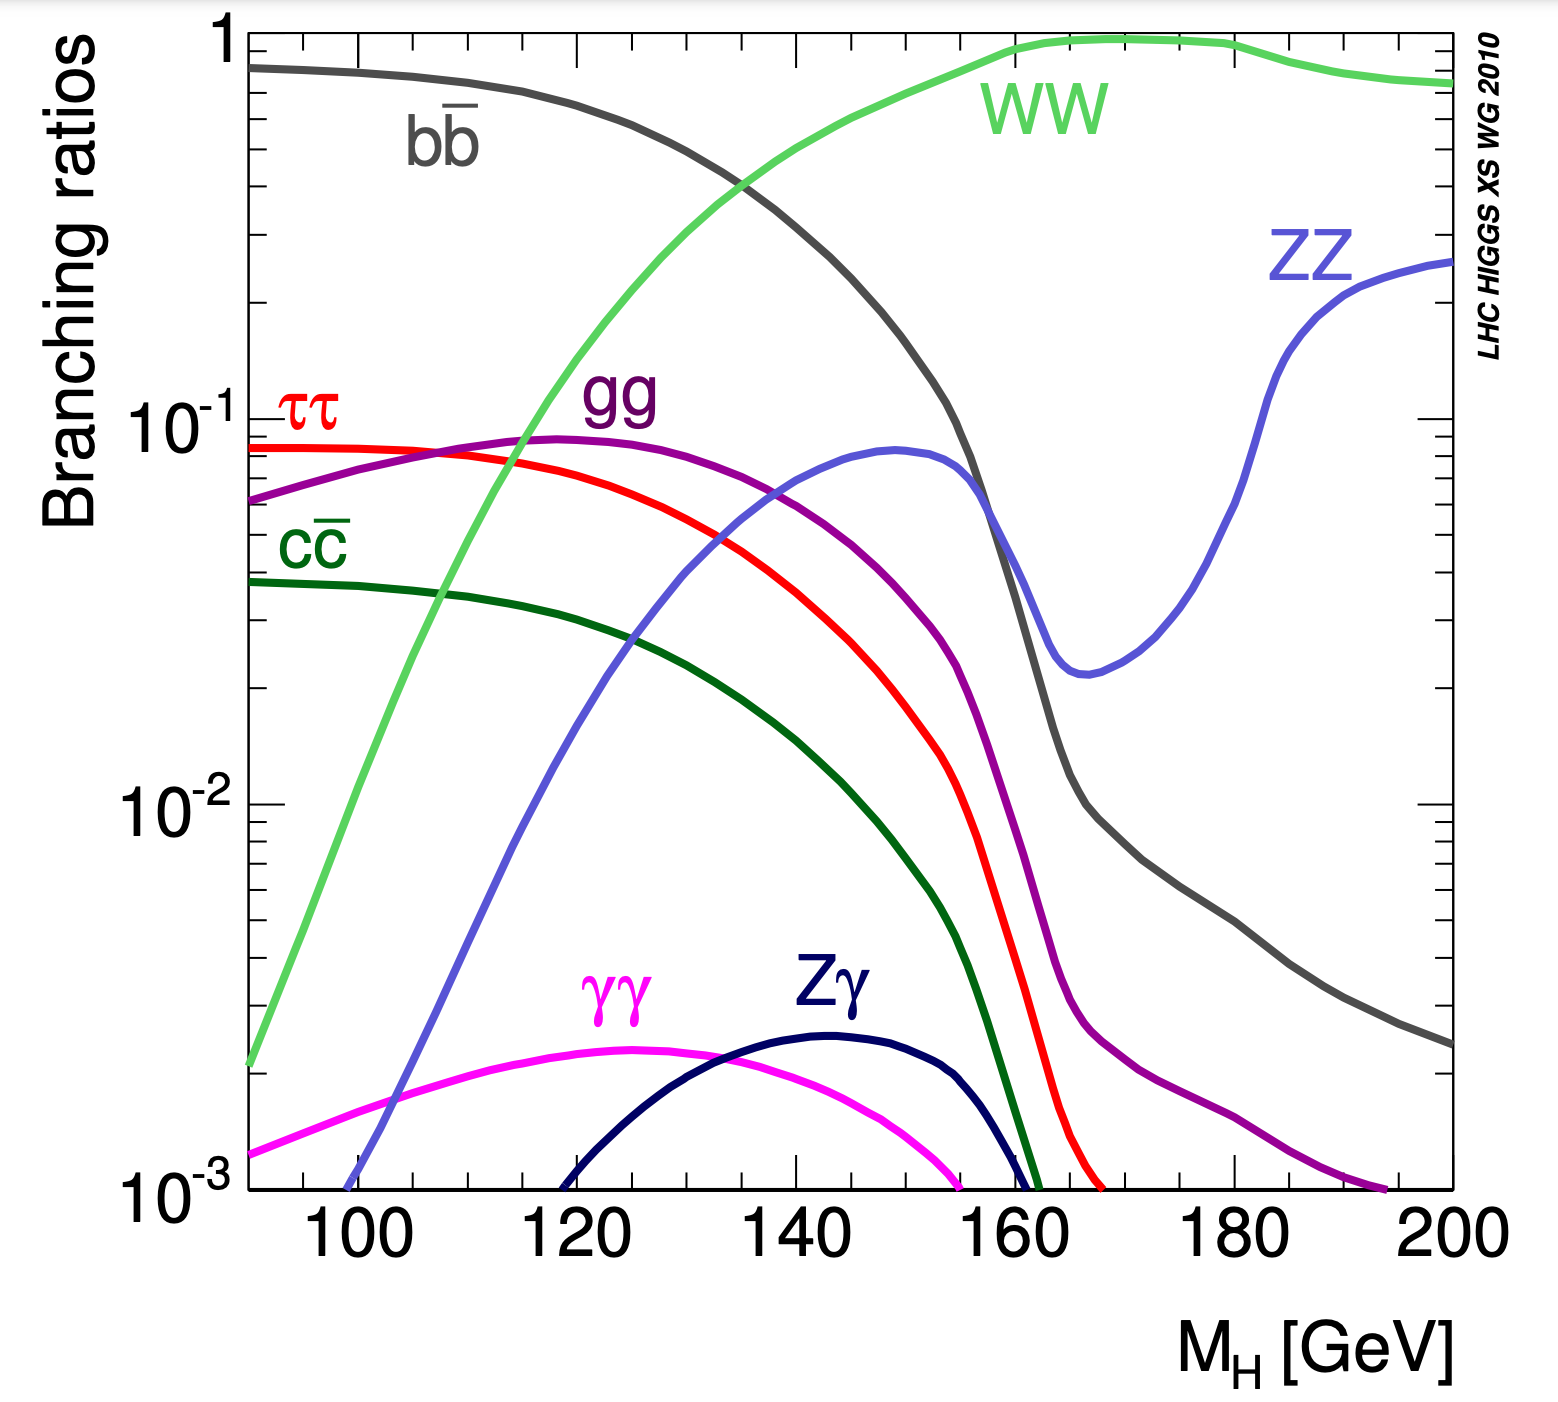
\includegraphics[height=10cm, width=12cm]{pictures/XS-MH.png}
  \caption{希格斯衰变分支比关于希格斯质量的函数关系}
 \label{fig:2.5}
\end{figure}
同时,这张图也暗示了除了标准模型希格斯粒子之外其他可能的WW共振态的衰变信息。

\begin{figure}[H]
 \centering
 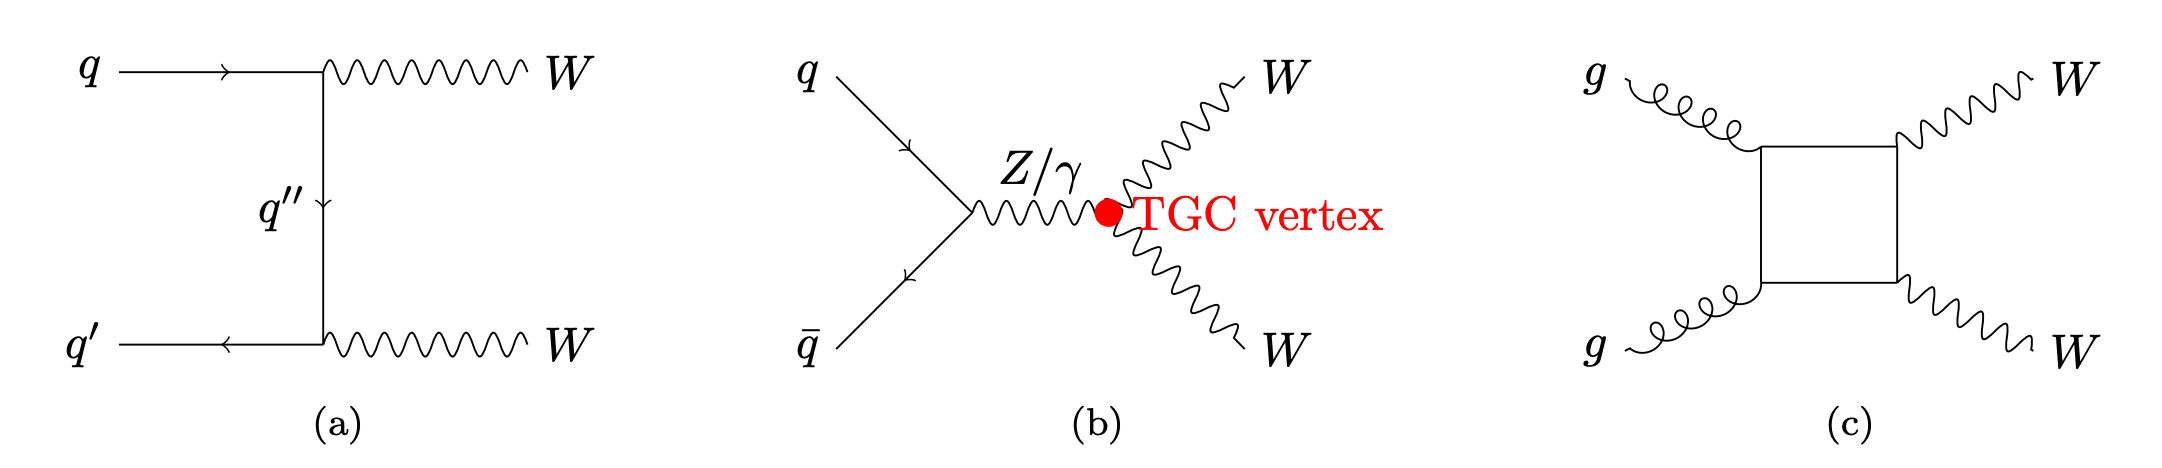
\includegraphics[height=4cm, width=16cm]{pictures/WW_bkg.png}
  \caption{非共振态$WW$的主要产生过程:(a)$qq^\prime\to WW$的t通道图;(b)$qq^\prime\to WW$的s通道图,有一个三规范玻色子耦合顶点(TGC);(c)$gg\to WW$的box图,贡献被LHC的高亮度胶子抬高。}
 \label{fig:2.6}
\end{figure}

$H\to WW^*$的主要本底来自于标准模型下的非共振WW生产道连续谱。在LHC上,WW生产过程由$q\bar{q}$湮灭过程主导,如图所示:左边和中间分别是$qq^\prime\to WW$过程的t通道图、s通道图,其中s通道过程对于$WWZ$和$WW\gamma$的三玻色子耦合顶点十分敏感。次领头阶的WW本底还有如右边所示的胶子聚合(ggF)生成WW的box图,尽管是次领头阶图,但这个过程被LHC上的高亮度胶子产物增强,从而对非共振态WW的产生贡献也不可忽视。

WW过程是LHC上第一批可观测到的双玻色子末态之一。总的来说,双玻色子产生提供了在TeV尺度检验标准模型电弱理论的机会。WW过程就是其中重要的一个例子。除此之外,WW产生过程还对三玻色子耦合顶点十分敏感,从而提供了检验标准模型规范对称性(与三玻色子耦合的限制有关)的重要机会。通过对WW产生过程的三玻色子耦合的精确测量,我们有机会探寻到包含规范玻色子的新物理现象。以及最重要的,对希格斯粒子的精确测量。


HWW道的测量还有助于研究各种新物理模型

\begin{figure}[H]
 \centering
 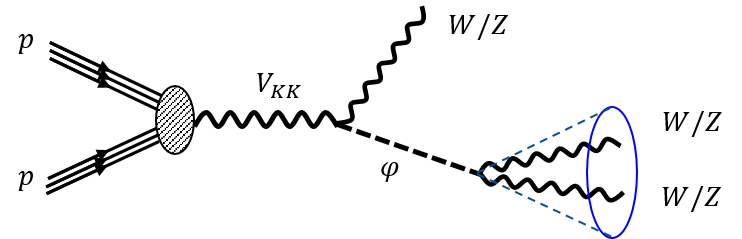
\includegraphics[height=5cm, width=16cm]{pictures/Vkk.png}
  \caption{可考虑的超出标准模型物理过程,基于扭曲的额外维RS模型的扩展。$V_{kk}$表示$W/Z$的Kaluza-Klein(KK)模式,并且对应于较重的母粒子。$\phi$表示标量粒子,被认为是标准模型中的EW规范玻色子。两个$W/Z$粒子周围来自$\phi$衰变的圆锥体表明它们是高度准直的。}
 \label{fig:2.7}
\end{figure}

\begin{figure}[H]
 \centering
 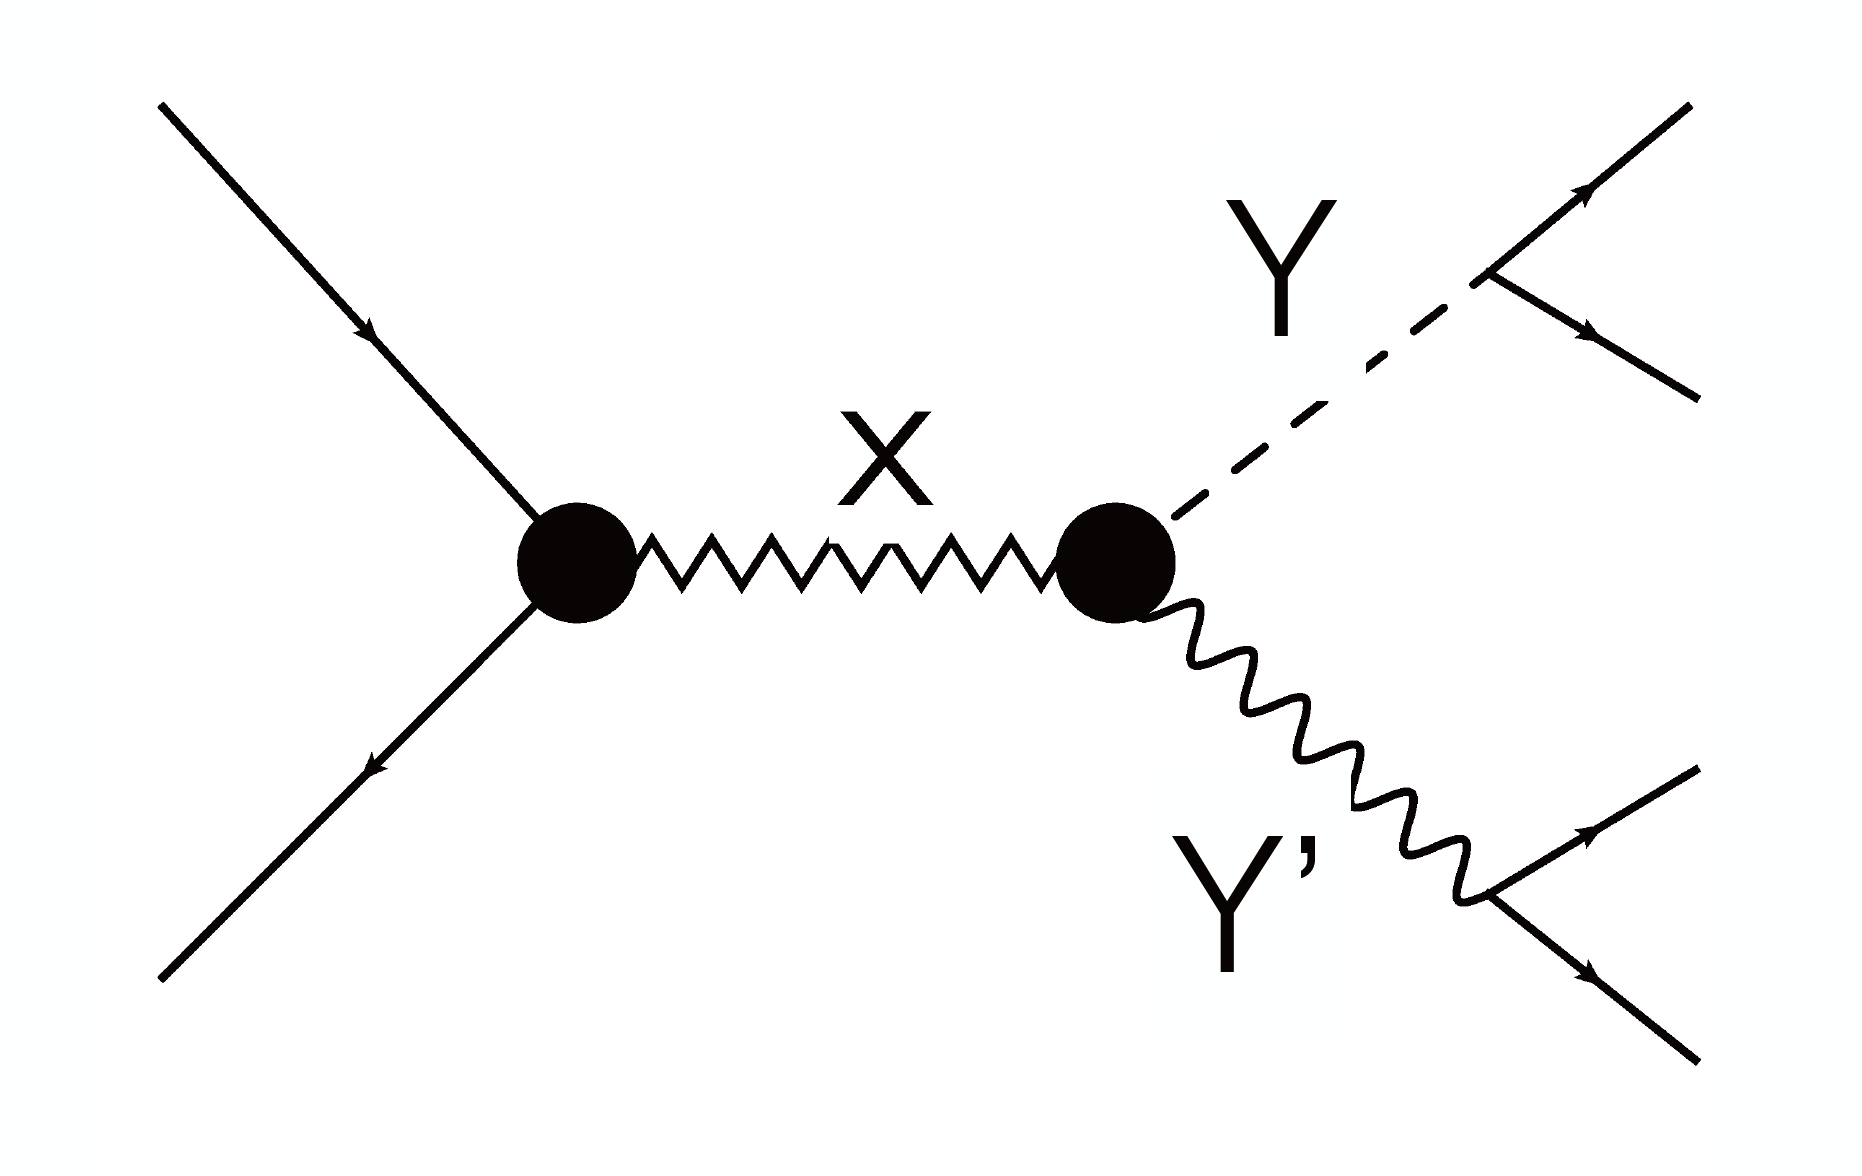
\includegraphics[height=6cm, width=10cm]{pictures/diboson_resonance_X.png}
  \caption{$X$代表TeV能量尺度的新物理粒子,$Y/Y^\prime$是$W/Z/H$玻色子。}
 \label{fig:2.7}
\end{figure}
可以通过探寻类似上图的过程,寻找可能的额外维度拉格朗日项,复合的希格斯粒子,扩展的规范对称性(更多类型的$Z/W$玻色子)
